% !TeX root = ../defense.tex

\section{Evaluation}
\frame{\sectionpage}

\begin{frame}[fragile]{Linear Road Data}
Query Type, Time stamp, vehicle ID, speed, expressway, lane, direction, segment, position, query ID, start segment, end segment, day of week, minute of day, day in past 10 weeks
\begin{lstlisting}[caption= Example of Linear Road Data]
0,0,13,10,8,0,0,89,469920,-1,-1,-1,-1,-1,-1
0,0,17,10,8,0,1,65,348479,-1,-1,-1,-1,-1,-1
0,0,22,10,8,0,0,12,63360,-1,-1,-1,-1,-1,-1
0,0,33,10,8,0,1,94,501599,-1,-1,-1,-1,-1,-1
0,0,42,10,8,0,0,14,73920,-1,-1,-1,-1,-1,-1
0,0,4,10,7,0,0,61,322080,-1,-1,-1,-1,-1,-1
0,0,85,10,8,0,1,30,163679,-1,-1,-1,-1,-1,-1
0,0,11,10,6,0,1,41,221759,-1,-1,-1,-1,-1,-1
0,0,23,10,7,0,1,81,432959,-1,-1,-1,-1,-1,-1
0,0,15,10,6,0,0,5,26400,-1,-1,-1,-1,-1,-1
\end{lstlisting}
\end{frame}


\begin{frame}{Data Distribution}
    \begin{figure}
        \centering
        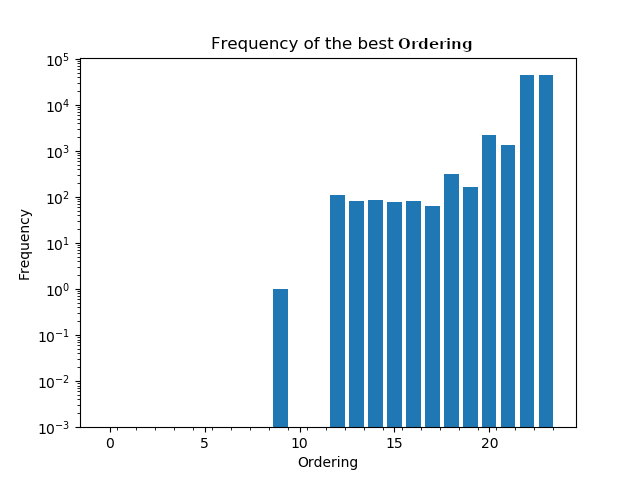
\includegraphics[scale=0.45]{totalb1.png}\\
        \caption{Shows for each ordering of operations, the number of data windows for which it was optimal, the data is baised towards the last 2 orderings.}
        \label{fig:totalb1}
    \end{figure}
\end{frame}


\begin{frame}{Data Distribution}
    \begin{figure}
        \centering
        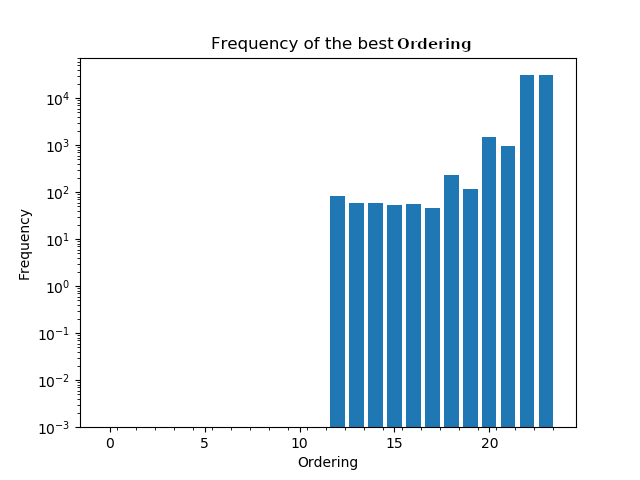
\includegraphics[scale=0.45]{trainingb1.png}\\
        \caption{Shows for each ordering, the number of data windows in trainging data for which it was optimal, the data was divided into 70\%:30\% for training and testing}
        \label{fig:trainingb1}
    \end{figure}
\end{frame}

\begin{frame}{Data Distribution}
    \begin{figure}
        \centering
        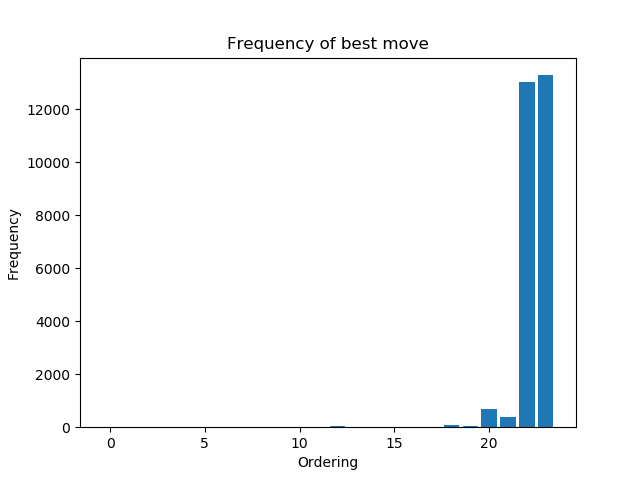
\includegraphics[scale=0.45]{testingb1.png}\\
        \caption{Shows for each ordering, the number of data windows in testing data for which it was optimal, the data was divided into 70\%:30\% for training and testing}
        \label{fig:testingb1}
    \end{figure}
\end{frame}

\begin{frame}[fragile]{Confusion Matrix}
    \begin{lstlisting}[caption=Confusion matrix for DQN classificaiton, label={lst:confusion_matrix}]
        [[   0    0    0    0    0    0    0    0    0    0    0    1    0]
         [   0    0    0    0    0    0    0    0    0    0    0   16   13]
         [   0    0    0    0    0    0    0    0    0    0    0   18    5]
         [   0    0    0    0    0    0    0    0    0    0    0   13   12]
         [   0    0    0    0    0    0    0    0    0    0    0   12   13]
         [   0    0    0    0    0    0    0    0    0    0    0   17    6]
         [   0    0    0    0    0    0    0    0    0    0    0    9    9]
         [   0    0    0    0    0    0    0    0    0    0   10   21   49]
         [   0    0    0    0    0    0    0    0    0    3    4   13   26]
         [   0    0    0    0    0    0    0    1    0   18   77  213  374]
         [   0    0    0    0    0    0    0    0    0   19   69  118  195]
         [   0    0    2    0    0    0    0    0    0  116  406 6347 6167]
         [   0    0    1    0    0    0    0    6    0  113  476 6338 6355]]
    \end{lstlisting}
\end{frame}

\begin{frame}{Confusion Matrix}
    The predictions on trained model lead to the following confusion matrix.
    \begin{figure}
        \centering
        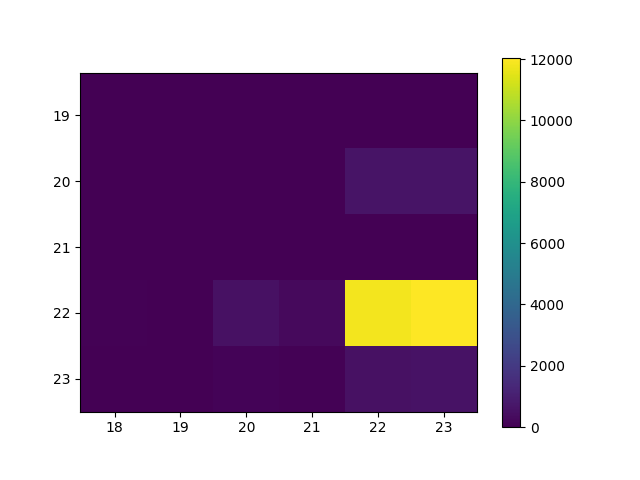
\includegraphics[scale=0.3]{cm3.png}\\
        \caption{DQN predictions visualized as confusion matrix}
        \label{fig:dqn_r2_1}
    \end{figure}
\end{frame}

\begin{frame}{Predictions}
    Some of the cases we were able to predict the correct answers.
    \begin{figure}
        \centering
        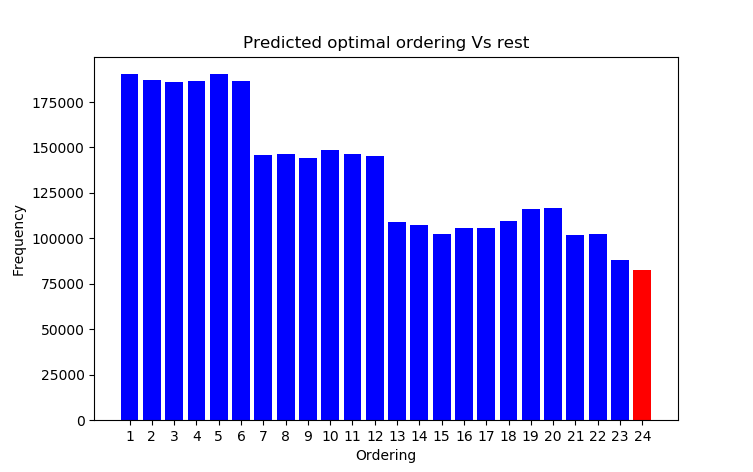
\includegraphics[scale=0.4]{operations1.png}\\
        \caption{The figure shows the log$_{10}$(number of operations) required to execute the query depending on the ordering of the selection operators chosen. The predicted optimal ordering is shown in red.}
        \label{fig:operations1}
    \end{figure}
\end{frame}

\begin{frame}{Predictions}
    Some of the cases we were able to predict the correct answers.
    \begin{figure}
        \centering
        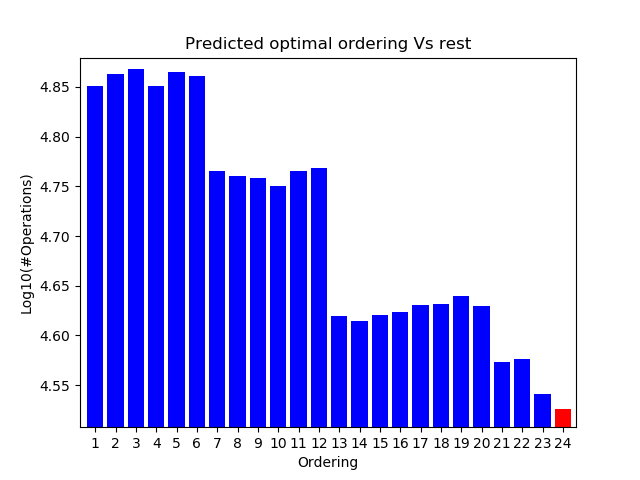
\includegraphics[scale=0.4]{operations2.png}\\
        \caption{The figure shows the log$_{10}$(number of operations) required to execute the query depending on the ordering of the selection operators chosen. The predicted optimal ordering is shown in red.}
        \label{fig:operations2}
    \end{figure}
\end{frame}



